\documentclass[12pt,letterpaper]{article}
\usepackage[utf8]{inputenc}
\usepackage{amsmath,amssymb,fullpage,graphicx}
\usepackage{subfigure}
\let\hat\widehat
\let\tilde\widetilde


\author{Nan Tang \\ 1662478}
	%% your name
\title{STAT 403 Spring 2018\\HW08}
	%% title of this document
\begin{document}
\maketitle

\section*{Q1}
\subsection*{Q1-a}
\begin{align*}
bias(\hat{g_n} (x_0)) &= E(\hat{g_n} (x_0)) - g(x_0) \\
&= E(\hat{p_n}^{\prime} (x_0)) - p^{\prime} (x_0) \\
&= \frac{1}{h} E(K^{\prime}(\frac{x - x_0}{h})) - p^{\prime} (x_0) \\
&= \frac{1}{h} \int K^{\prime}(\frac{x - x_0}{h}) p(x) dx - p^{\prime} (x_0) \\
\end{align*}
\noindent change variable such that $y = \frac{x-x_0}{h}$, then $dy = \frac{dx}{h}$, $K^{\prime}(\frac{x-x_0}{h}) = K^{\prime}(y)/h$
\begin{align*}
bias(\hat{g_n} (x_0)) &= \frac{1}{h} \int K^{\prime}(y) p(x_0 + hy) dy - p^{\prime} (x_0)
\end{align*}

\noindent By Taylor expansion, when h is small, 
\begin{align*}
p(x_0 + hy) &= p(x_0) - hy \cdot p^{\prime} (x_0) + \frac{1}{2} h^2 y^2 p^{\prime \prime}(x_0) + \frac{1}{3 !}h^3 y^3 p^{\prime\prime\prime}(x_0) + o(h^3)
\end{align*}
\begin{align*}
bias(\hat{g_n} (x_0)) &= \frac{1}{n}[ p(x_0)\int K^{\prime}(y) dy +  h p^{\prime}(x_0) \int yK^{\prime}(y) dy \\
&+  \frac{h^2 p^{\prime\prime}(x_0)}{2} \int  y^2 K^{\prime} (y)dy   + \frac{h^3 p^{\prime\prime\prime}(x_0)}{6} \int y^3 K^{\prime}(y) dy + o(h^2)] - p^{\prime} (x_0)
\end{align*}

\noindent Since $K^{\prime}$ the derivative of standard normal is and odd function, $\int K^{\prime}(y) dy, \int  y^2 K^{\prime} (y)dy$ are equal to zero.\\

\noindent $\int y K^{\prime}(y) dy = [yK(y)] - \int K(y) dy = 0 - 1$

\begin{align*}
bias(\hat{g_n} (x_0)) &= p^{\prime}(x_0) + h^2 \frac{p^{\prime\prime\prime}(x_0)}{6} \int y^3 K^{\prime}(y) dy + o(h^2) - p^{\prime}(x_0) \\
&= C_1 h^2 + o(h^2) \text{, where C1 is a constant} 
\end{align*}

\begin{align*}
Var(\hat{g_n} (x_0)) &= Var(\hat{p_n}^{\prime} (x_0)) \\
&= \frac{1}{nh^2}Var(K^{\prime}(\frac{x - x_0}{h})) \\
&\leq  \frac{1}{nh^2} E(K^{\prime}(\frac{x-x_0}{h})^2) \\
&= \frac{1}{nh^2} \int K^{\prime}(\frac{x-x_0}{h})^2 p(x) dx
\end{align*}
\noindent change variable such that $y = \frac{x-x_0}{h}$, then $dy = \frac{dx}{h}$, $K^{\prime}(\frac{x-x_0}{h})^2 = K^{\prime}(y)^2/h^2$
\begin{align*}
Var(\hat{g_n} (x_0)) &\leq \frac{1}{nh^3} \int K^{\prime}(y) p(x_0 + hy) dy\\
&= \frac{1}{nh^3} \int K^{\prime}(p(x_0)^2 + hyp^{\prime} (x_0) + o(h)) dy 
\end{align*}
\noindent Note that $ \int K^{\prime}(y) y dy = 0$ since $K$ is an odd function.
\begin{align*}
Var(\hat{g_n} (x_0)) &\leq \frac{1}{nh^3} p(x_0) \int K^{\prime}(y)^2 dy + o(\frac{1}{nh^3}) \\
&= \frac{C_2}{nh^3} + o(\frac{1}{nh^3})
\end{align*}

\subsection*{Q1-b}
\begin{align*}
bias(\hat{p_n}(0)) &= E(\hat{p_n}(0)) - p(0) \\
&= E(\frac{1}{nh} \sum K(\frac{x_i - 0}{h})) - p(0) \\
&= \frac{1}{h} \int K(\frac{x}{h}) p(x) dx - p(0)
\end{align*}
\noindent Note that $p(0) = 0$ and $p(x) = 2x$ when $0 \leq x \leq 1$, otherwise $p(x) = 0$
\begin{align*}
bias(\hat{p_n}(0)) &= \frac{1}{n} \int_{0}^{1} K(\frac{x}{h}) 2x dx \\
&= \frac{1}{n} \int_{0}^{1} \frac{1}{\sqrt{2 \pi}} e^{\frac{-x^2}{2h^2}} 2x dx \\
&= \frac{1}{h} \cdot \frac{2}{\sqrt{2 \pi}} \int_{0}^{1} e^{\frac{-x^2}{2h^2}}  x dx \\
&= \frac{2}{h \sqrt{2 \pi}} [-h^2 (e^{-\frac{1}{2h^2}} - 1) + o(h^2)] \\
&= -\frac{2h}{\sqrt{2\pi}}e^{-\frac{1}{2h^2}} + o(h) \\
\end{align*}
\noindent  let $C_3 = -\frac{2}{\sqrt{2\pi}}e^{-\frac{1}{2h^2}}$, $e^{-\frac{1}{h^2}} < 1$, $C_3$ is a constant. 
\begin{align*}
bias(\hat{p_n}(0)) &= C_3 h + o(h)
\end{align*}

\subsection*{Q1-c}
\noindent The CDF of $X^{\star}_i$, $F(x)$ can be represented as
\begin{align*}
F(x) &= P(X^{\star}_i \leq x) \\
&= P(Y^{\star}_i + Z_i \leq x) \\
\end{align*}
\noindent $Y^{\star}_i$ is bootstrapped from $X_1...X_n$, therefore, probability of $Y^{\star}_i = X_i$ is equal to $\frac{1}{n}$ (each $X_i $ has equal chance be bootstrapped)

\begin{align*}
F(x) &=  \sum_{i=1}^n \frac{P(Y^{\star}_i + Z_i \leq x | Y^{\star}_i = x_i)}{P(Y^{\star}_i = x_i)} \\
&= \frac{1}{n} \sum_{i=1}^n P(x_i + Z_i \leq x) \\
&= \frac{1}{n} \sum_{i=1}^n P(Z_i \leq x - x_i)
\end{align*}
\noindent $Z_i \sim N(0, h^2)$, therefore, $P(Z_i \leq x - x_i) = \Phi(\frac{x-x_i}{h})$
\begin{align*}
f_{X^{\star}_i}(x) &= dF(x) / dx \\
&=  (d(\frac{x - x_i}{h})/dx) \cdot  \frac{1}{n} \sum_{i=1}^n K(\frac{x - x_i}{h}) \text{ where K is pdf of standard normal} \\
&= \frac{1}{nh} \sum K(\frac{x - x_i}{h}) 
\end{align*}
\noindent Since K is a symmetric function around zero, $K(\frac{x-x_i}{h}) = K(\frac{x_i - x}{h})$. \\

\noindent Therefore, PDF of $X^{\star}_i = \frac{1}{nh} \sum K(\frac{x_i - x}{h})$ which is equal in density to KDE function.


\subsection*{Q1-d}
\begin{align*}
\hat{p_n}(x_0) &= \frac{1}{nh} \sum K(\frac{x_i - x_0}{h}) \\
&= \sum K(\frac{x_i - x_0}{h}) \text{, since } h = \frac{1}{n} \\
&= \sum \frac{1}{2} I(-1 \leq \frac{x_i - x_0}{h} \leq 1) \\
2\hat{p_n}(x_0) &= \sum I(-1 \leq \frac{x_i - x_0}{h} \leq 1) \\
&=  \sum I(-h + x_0 \leq x_i \leq h + x_0)
\end{align*}

\noindent $\sum I(-h + x_0 \leq x_i \leq h + x_0)$ is total number of observations that falls in interval $[-h + x_0 , h + x_0]$. \\

\noindent For random variables $x_1, x_2 ... x_n$, let $q_n$ denotes the probability of $x_i$ falls in interval $[-h + x_0 , h + x_0]$. \\

\noindent $nq_n$ denotes number of $x_i$'s falls in the interval, which depends on $x_0$ and $h$, when $n \rightarrow \infty$, $h \rightarrow 0$, so $nq_n$ only depends on $x_0$ when $n$ is large enough. \\

\noindent Let $\lambda(x_0)$ denotes function of $x_0$ only. When n is large enough, $nq_n \rightarrow \lambda(x_0)$, and by law of small number, $x_n \rightarrow Poi(\lambda(x_0))$ in distribution. \\

\noindent In this case, $x_n$ is $2 \hat{p_n}(x_0)$, therefore, $2 \hat{p_n}(x_0) \rightarrow Poi(\lambda(x_0))$ in distribution. 

\newpage
\section*{Q2}
\subsection*{Q2-a}
\begin{verbatim}
eruption_dt <- faithful$eruptions

bwds <- c(0.1, 0.3, 0.9)
colors <- c('red', 'blue', 'green')
plot(1, type="n", xlab="Eruption", ylab="Density", xlim=c(min(eruption_dt), max(eruption_dt)),
     ylim=c(0, 1), main='KDE Function of Eruption')
for (ii in 1:length(bwds)) {
  erupt_kde <- density(eruption_dt, bw=bwds[ii])
  lines(erupt_kde, lwd=3, col=colors[ii])
}
legend('topright', legend=c('bw=0.1', 'bw=0.3', 'bw=0.9'), col=colors, lwd=3, cex=0.8)
\end{verbatim}

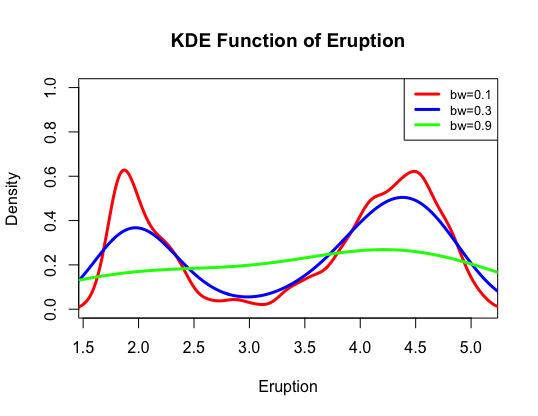
\includegraphics[scale=0.7]{q2-a.png}

\subsection*{Q2-b}
\begin{verbatim}
erupt_kde <- density(eruption_dt, bw=0.3)
hist(eruption_dt, breaks=20, probability=T)
lines(erupt_kde, lwd=3)
\end{verbatim}

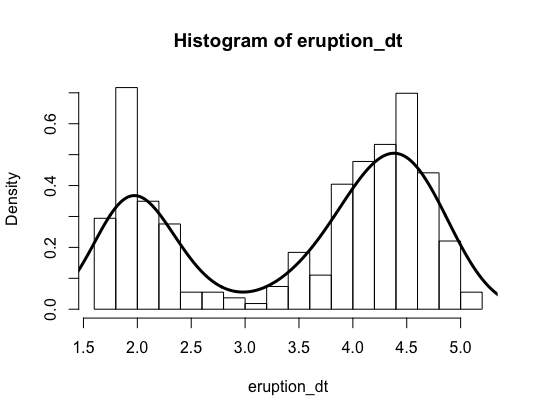
\includegraphics[scale=0.7]{q2-b.png}

\subsection*{Q2-c}
\begin{verbatim}
erupt_kde <- density(eruption_dt, from=1, to=6, bw=0.3)
n <- length(eruption_dt)
B <- 10000
kde_bt <- matrix(NA, B, length(erupt_kde$x))
for (ii in 1:B) {
  sp_index <- sample(n,n,replace=T)
  sp_bt <- eruption_dt[sp_index]
  sp_kde <- density(sp_bt, from=1, to=6, bw=0.3)
  kde_bt[ii,] <- sp_kde$y
}

bt_sd <- sqrt(diag(var(kde_bt)))

plot(erupt_kde, lwd=3, col="blue", ylim=c(0,0.6),main="95% CI of KDE Function")
lines(x=erupt_kde$x,y=erupt_kde$y+qnorm(0.975)*bt_sd, lwd=3, col="dodgerblue",
      lty=2)
lines(x=erupt_kde$x,y=erupt_kde$y-qnorm(0.975)*bt_sd, lwd=3, col="dodgerblue",
      lty=2)
\end{verbatim}

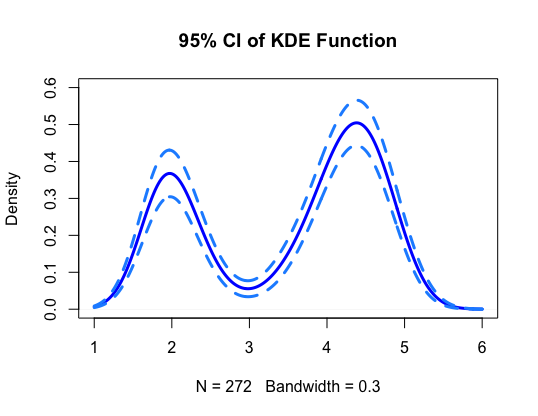
\includegraphics[scale=0.7]{q2-c.png}

\section*{Q3}
\subsection*{Q3-a}
\begin{verbatim}
library(smoothmest)
n=1000
dexp_dt <- rdoublex(n, mu=0, lambda=1)
dexp_den <- density(dexp_dt, bw=0.2, from=-6, to=6, n=n)
x_base <- dexp_den$x
dexp_true <- ddoublex(x_base, mu=0, lambda=1)

plot(x=x_base, y=dexp_den$y, type='l', lwd=3, col='skyblue', xlim=c(-6,6), 
     ylim=c(0, 0.5), xlab='X', ylab='Density', main='KDE of 1000 R.N from Double Exponential')
lines(x=x_base, y=dexp_true, lwd=3, lty=3, col='coral1')
legend('topright', legend=c('KDE h=0.2', 'dexp lambda=1'), col=c('skyblue', 'coral1'), 
       lty=c(1,2), lwd=2, cex=0.8)
\end{verbatim}
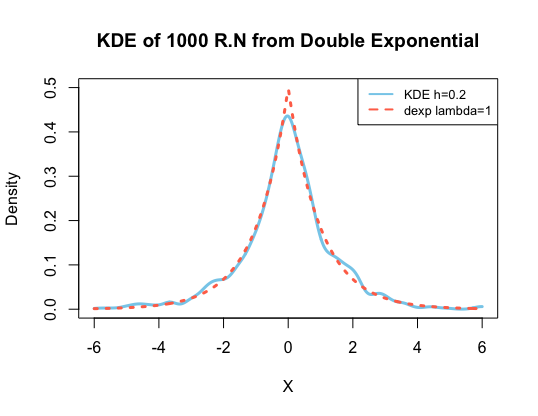
\includegraphics[scale=0.7]{q3-a.png}

\subsection*{Q3-b}
\noindent In this case, both bias and variance cause KDE unmatch to true density. We can perceive from the plot in previous question that true density has a sharp turning (peaked bump) near zero, meanwhile, density value around zero is much higher than at other regions. Large bias appears at sharp turning point, while large variance appears at where density is large. Points around zero satisfy both conditions, therefore, large bias and large variance together caused the discrepancy at zero. 

\subsection*{Q3-c}
\begin{verbatim}
N = 10000
bwds <- seq(0.05, 0.5, 0.05)

mise_result <- rep(NA, length(bwds))
for (ii in 1:length(bwds)) {
  bwd <- bwds[ii]
  kde_result <- matrix(NA, nrow=N, ncol=n)
  for (jj in 1:N) {
    temp_den <- density(dexp_dt, from=-6, to=6, n=n, bw=bwd)
    kde_result[jj,] <- temp_den$y
  }
  mse_result <- colSums((t(t(kde_result) - dexp_true))^2) /N
  mise_result[ii] <- sum(mse_result)
}

plot(x=bwds, y=mise_result, pch=16, xlab='Bandwidth', ylab='MISE', 
     main='Bandwidth vs MISE', col='coral1')
lines(x=bwds, y=mise_result, lwd=2, col='skyblue')

opt_bwd <- bwds[which.min(mise_result)]
> opt_bwd
[1] 0.2
\end{verbatim}

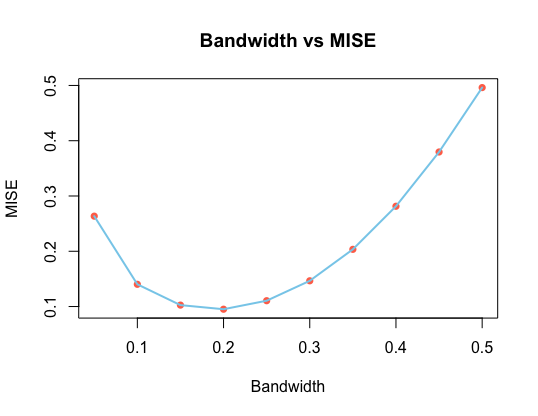
\includegraphics[scale=0.7]{q3-c.png}

\noindent MISE minimized when choosing bandwidth 0.2

\end{document}